% Camera-ready source, MLMI 2026 (Paper 35).
% Compile with pdflatex (Springer LNCS class, llncs.cls).
% Overleaf: New Project -> Springer -> Lecture Notes in Computer Science,
% then replace main.tex with this file and upload the figures/ directory.
\documentclass[runningheads]{llncs}

\usepackage[T1]{fontenc}
\usepackage[utf8]{inputenc}
\usepackage{graphicx}
\usepackage{booktabs}
\usepackage{amsmath}
\usepackage{amssymb}
\usepackage{siunitx}
\usepackage[hidelinks]{hyperref}
\usepackage{url}

\sisetup{detect-weight=true, detect-family=true}
\renewcommand{\arraystretch}{1.12}

\begin{document}

\title{Leakage-Controlled Resting-State Connectome Classification of
Schizophrenia: A Nested Cross-Validation Audit of the COBRE Cohort}

\titlerunning{Leakage-Controlled Connectome Classification of Schizophrenia}

\author{Ishsirjan Kaur Chandok}
\authorrunning{I. K. Chandok}
\institute{Institut de G\'en\'etique Mol\'eculaire de Montpellier, CNRS UMR 5535,\\
1919 Route de Mende, 34293 Montpellier Cedex 5, France\\
\email{ishsirjanchandok.iskc@gmail.com}}

\maketitle

\begin{abstract}
Resting-state functional connectomes are widely used to discriminate patients with
schizophrenia from healthy controls, yet reported cross-validated accuracy depends
heavily on the point at which features are defined relative to the train/test split.
We audit this dependence on 146 participants of the COBRE cohort parcellated with the
Schaefer-100 atlas (4,950 edges). Exploratory covariate-adjusted mass-univariate
inference is kept strictly separate from prediction, and every predictive pipeline
performs edge screening, dimensionality reduction and hyperparameter search inside the
outer training folds of a repeated nested cross-validation. Under this regime,
elastic-net logistic regression reaches an AUC of $0.768 \pm 0.076$ and PCA-30 an AUC of
$0.771 \pm 0.079$, with an edges-only elastic net essentially unchanged at
$0.765 \pm 0.079$. Fold-wise residualisation of mean framewise displacement lowers that
edges-only estimate to 0.694. Holding a twenty-edge $|t|$ screen and a logistic classifier
fixed, and varying only whether the screen sees the test fold, isolates leakage for that
construction: AUC rises from $0.709 \pm 0.076$ to $0.903 \pm 0.039$. That 0.194 gap is the
cost of leaking a hard univariate screen, not of leaking the primary elastic net. The
same construction on a 50/50 age-, sex- and FD-matched subsample of UCLA CNP yields
0.679 against 0.873, again a 0.194 gap; that analysis is within-cohort nested
cross-validation, not a locked transfer, and does not revise 0.77. On synthetic data with no
signal the leakage-free protocol returns chance, whereas a leaked twenty-edge screen
reports 0.82 when the edges are correlated as in a connectome and 0.94 when they are
independent; the observed leaked value of 0.903 lies between those bounds and about 0.08
above the correlated floor. Calibration and subject-level
aggregation of repeated out-of-fold predictions are reported for the leakage-free model.
The resulting figure of roughly 0.77 AUC is specific to this cohort, parcellation,
connectivity measure and model family rather than a general ceiling, and the audit
protocol is released as public code.

\keywords{Functional connectivity \and Cross-validation \and Data leakage \and
Schizophrenia \and Validation protocol}
\end{abstract}

\section{Introduction}

Machine learning applied to functional neuroimaging is increasingly proposed as a route
to computer-aided diagnosis in psychiatry~\cite{Arbabshirani2017,Wolfers2015}.
Schizophrenia is associated with altered resting-state functional connectivity,
particularly across default-mode, salience and frontoparietal
systems~\cite{Fornito2015,Menon2011,Woodward2015}, and a full pairwise connectome
supplies thousands of candidate features from a single scan. The apparent accuracy of a
connectome classifier, however, is determined as much by the validation protocol as by
the biology it is meant to capture.

A frequent pipeline screens edges on the whole cohort, retains the significant
connections, and only then trains a classifier that is evaluated by cross-validation.
Selection performed at that point encodes label information from participants who will
later serve as test cases, and nesting the classifier alone cannot remove the resulting
optimism~\cite{Arbabshirani2017,Varoquaux2017}. The distinction between exploratory
group-level inference and predictive feature construction is therefore not a stylistic
one: the two answer different questions and require different guarantees.

We quantify that distinction on the public COBRE cohort~\cite{Aine2017}.
Our contributions are fivefold. First, we report a leakage-free benchmark in which
elastic net, principal component analysis, connectome-based predictive
modelling~\cite{Shen2017}, per-fold univariate screening and network-level aggregation
are all fitted inside the outer training folds of a repeated nested cross-validation.
Second, we separate a covariate-adjusted exploratory map from every predictive pipeline.
Third, we isolate the leakage effect with a contrast in which the selector, the
classifier and the hyperparameter grid are identical and only the scope of the edge
screen changes; this distinguishes optimism caused by leakage from optimism caused by a
different model. Fourth, we examine head motion, probability calibration and the
aggregation of repeated out-of-fold predictions, which jointly determine how the honest
estimate should be interpreted. Fifth, we repeat the matched contrast within the UCLA CNP
schizophrenia sample under a different preprocessor, and on signal-free synthetic
connectomes. UCLA CNP is balanced by 1:1 nearest-neighbour matching on age, sex and mean
FD (50/50) and is analysed with within-cohort nested cross-validation, not a
train-on-COBRE transfer. Code and split definitions are publicly available.

\begin{figure}[t]
\centering
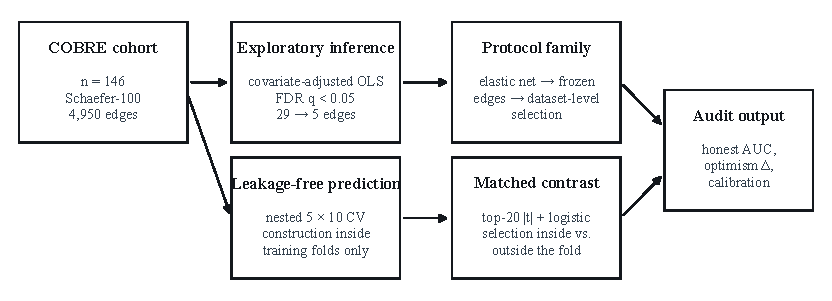
\includegraphics[width=\textwidth]{figures/fig1_design.pdf}
\caption{Design of the audit on COBRE. Group-level inference and predictive modelling are kept
separate. Every leakage-free pipeline fits its feature construction inside the outer
training folds. Two comparisons then relax that constraint: a mixed protocol in which
the feature space also changes, and a matched contrast in which only the scope of the
edge screen changes.}
\label{fig:design}
\end{figure}

\section{Materials and Methods}

\subsection{Data and Preprocessing}
We used the publicly released COBRE resting-state fMRI collection (Figshare acquisition
4197885), preprocessed with the NIAK pipeline~\cite{Aine2017,Bellec2012}. Participants
were retained when both the preprocessed BOLD volume and the accompanying confound time
series were available, giving 146 individuals. The distributed phenotypic file provides
age, sex and mean framewise displacement (FD); no symptom inventories were available, so
the analysis concerns diagnostic classification only. All numeric confound regressors
were passed to the Nilearn \texttt{NiftiLabelsMasker} during parcel-wise signal
extraction with standardisation enabled~\cite{Abraham2014}. Parcellation used the
Schaefer 2018 atlas with 100 parcels under the seven-network Yeo solution at
\SI{2}{\milli\metre}~\cite{Schaefer2018,Yeo2011}, resampled to each subject's BOLD grid
by nearest-neighbour interpolation.

\subsection{Connectivity Estimation}
Pearson correlations between all pairs of parcel time series produced one
$100 \times 100$ symmetric matrix per participant. Discarding the diagonal and taking
the upper triangle yields 4,950 undirected edges, which were Fisher $z$-transformed
before modelling.

\subsection{Exploratory Group-Level Inference}
Two edge-wise procedures were applied to the full cohort for descriptive purposes.
Unadjusted two-sample $t$-tests with Benjamini--Hochberg control at
$q < 0.05$~\cite{Benjamini1995} identified 29 edges. A covariate-adjusted model,
\begin{equation}
\mathrm{FC}_{ij} = \beta_0 + \beta_1 \cdot \mathrm{diagnosis} + \beta_2 \cdot
\mathrm{age} + \beta_3 \cdot \mathrm{sex} + \beta_4 \cdot \mathrm{FD} + \epsilon ,
\end{equation}
was then fitted per edge and the false discovery rate was controlled on $\beta_1$. These
maps are reported as inference and were excluded from every leakage-free predictive
pipeline.

\subsection{Feature Construction under Fold Isolation}
Because feature construction rather than the classifier alone drives optimism, five
strategies were compared, each fitted exclusively on outer training indices: an
elastic-net logistic regression over all 4,950 edges; a 30-component PCA;
connectome-based predictive modelling summarising the top and bottom decile of
training-fold edge correlations into two scores~\cite{Shen2017}; the twenty edges with
the largest training-fold absolute $t$ statistic; and the 28 mean within- and
between-network Fisher $z$ values defined by the Yeo seven-network solution. Age, sex and
FD were optionally appended as measured covariates~\cite{Power2012}. Penalty paths and
component loadings were never estimated on held-out participants.

\subsection{Classifiers and Nested Validation}
Classifiers were implemented in scikit-learn~\cite{Pedregosa2011} and comprised
$L_2$-penalised logistic regression, an elastic-net logistic regression with the saga
solver, a radial-basis support vector machine and, for the network features, a random
forest. Each was wrapped in a standardisation pipeline, and hyperparameters were chosen
by an inner five-fold grid search maximising ROC-AUC. The outer loop was a stratified
five-fold partition repeated ten times, giving 50 outer splits. Fold-wise means and
standard deviations are reported as descriptive summaries; because the repeats overlap,
these standard deviations are not confidence intervals and are not used to rank methods
against each other. Secondary analyses that required out-of-fold
probabilities---subject-level aggregation, calibration, motion residualisation and the
matched leakage contrast---used five folds repeated three times; the elastic-net estimate
was stable between the two settings (0.770 versus 0.768).

\subsection{Aggregation of Repeated Out-of-Fold Predictions}
Under repeated cross-validation each participant contributes several test predictions.
Concatenating all of them treats repeated observations from the same individual as
independent. We therefore also computed a subject-level estimate in which the predicted
probabilities of each participant are averaged first and a single ROC-AUC is evaluated
over the 146 unique subjects. Both quantities are reported.

\subsection{Leakage Regimes}
Two families of comparison were run. The first contrasts the leakage-free elastic net
with a logistic regression restricted to the five covariate-adjusted edges of
Table~\ref{tab:edges}, whose identities come from full-cohort inference while only the
classifier is cross-validated. Because the feature space and the classifier differ, that
spread bounds mixed-protocol optimism and does not attribute it to leakage alone. A
dataset-level selection figure inherited from the accepted submission is not reported
here, because no released script regenerates it.

The second comparison isolates the selection step. The selector (the twenty largest
absolute $t$ statistics), the classifier ($L_2$ logistic regression), the covariate block
and the hyperparameter grid are held fixed, and the only difference is whether the screen
is computed within the outer training fold or on the complete cohort including the test
fold. Label permutation used 50 shuffles of the leakage-free protocol with
$p = (\#\{\mathrm{AUC}_{\mathrm{perm}} \geq \mathrm{AUC}_{\mathrm{obs}}\} + 1)/(n + 1)$;
the smallest attainable value is $1/51 \approx 0.02$, which bounds the resolution of this
test.

\subsection{Motion Sensitivity}
Mean FD differs between groups, so three analyses probe its contribution. An edges-only
elastic net omits the covariate block entirely. A residualisation variant regresses each
edge on FD using coefficients estimated on the training fold and applies the same
transformation to the test fold. Finally, five locked stratified 70/30 splits were
evaluated, with all feature construction confined to the training portion.

\subsection{Calibration and Coefficient Inspection}
Expected calibration error over ten equal-width bins and the Brier score were computed
from out-of-fold probabilities for the leakage-free models as well as for the leaked
contrast. Coefficients of the leaked reference logistic model were aggregated across
outer folds. Because that model draws on full-cohort edge identities and includes a
group-imbalanced motion covariate, its weights are reported as a description of what the
circular pipeline exploits and not as anatomical evidence.

\subsection{Matched Schizophrenia Sample and Null Control}
The matched contrast of Sect.~2.7 was repeated as nested cross-validation inside the
UCLA Consortium for Neuropsychiatric Phenomics rest sample (OpenNeuro
ds000030)~\cite{Poldrack2016}: 50 participants with schizophrenia who had an fMRIPrep MNI
rest series, each paired with one control by greedy nearest-neighbour matching on
standardised age, sex and mean FD (50/50). Time series used Schaefer-100 (4,950 edges);
numeric confound columns entered the masker; the same three covariates were appended.
This is within-CNP nested cross-validation under a different preprocessor, not a locked
transfer from COBRE, and it does not revise 0.77.

The second extra experiment removes the signal. Labels are random and features are
either independent Gaussians or connectomes built from random parcel time series with a
five-component latent structure (mean absolute correlation between edge pairs 0.10 at
the COBRE dimensions). For the CNP subsample we also permute the observed labels on the
real matched connectomes, which preserves the empirical edge dependence. Ten draws were
taken per configuration, including $k \in \{5, 20, 100\}$ and $n$ between 50 and 600 at
$p = 4{,}950$. A leakage-free protocol must return chance; whatever the leaked protocol
returns is the level its own design can manufacture with no signal.

\subsection{Implementation}
Analyses were run in Python 3.11 with Nilearn, NiBabel, SciPy, statsmodels and
scikit-learn~\cite{Abraham2014,Pedregosa2011}. Connectivity matrices, edge statistics,
benchmark tables and calibration summaries are exported as CSV. The audit protocol, the
split definitions and the analysis scripts are available at
\url{https://github.com/Ishsirjan/Leakage_Audit}; the imaging data remain at the original
Figshare and OpenNeuro records.

\section{Results}

\subsection{Sample and Exploratory Connectivity}
Table~\ref{tab:cohort} summarises the analysed sample. Patients moved more than controls
during acquisition (Welch $t = 4.33$, $p = 3.3 \times 10^{-5}$). Unadjusted testing
returned 29 FDR-significant edges; after adjustment for age, sex and FD only five
survived (Table~\ref{tab:edges}), a contraction consistent with the known influence of
micro-movements on connectivity estimates~\cite{Power2012}. The surviving connections
couple visual, salience/ventral-attention, default-mode and control systems
(Fig.~\ref{fig:connectome}), in line with large-scale network accounts of
psychosis~\cite{Menon2011}. They are reported as exploratory inference and were withheld
from the leakage-free pipelines.

\begin{table}[t]
\centering
\caption{Characteristics of the 146 analysed COBRE participants. FD denotes mean
framewise displacement in millimetres.}
\label{tab:cohort}
\begin{tabular}{lrrrr}
\toprule
Group & $N$ & Age (years) & Male, n (\%) & Mean FD \\
\midrule
Schizophrenia   & 72  & $38.2 \pm 13.9$ & 58 (80.6)  & $0.478 \pm 0.274$ \\
Healthy control & 74  & $35.8 \pm 11.6$ & 51 (68.9)  & $0.318 \pm 0.152$ \\
\midrule
Total           & 146 & $37.0 \pm 12.8$ & 109 (74.7) & $0.397 \pm 0.236$ \\
\bottomrule
\end{tabular}
\end{table}

\begin{table}[t]
\centering
\caption{Edges surviving false-discovery-rate control after adjustment for age, sex and
mean framewise displacement. These edges are exploratory and were not supplied to any
leakage-free predictive pipeline.}
\label{tab:edges}
\begin{tabular}{cllrr}
\toprule
\# & Parcel 1 & Parcel 2 & $t_{\mathrm{adj}}$ & $q_{\mathrm{FDR}}$ \\
\midrule
1 & LH Vis 3                     & RH Default Temp 2 & 4.38  & 0.031 \\
2 & LH SalVentAttn FrOperIns 1   & RH Default PFCv 1 & -4.93 & 0.011 \\
3 & LH Default Par 2             & RH Cont PFCl 1    & -4.30 & 0.031 \\
4 & RH Vis 8                     & RH Default Temp 2 & -4.33 & 0.031 \\
5 & RH SalVentAttn TempOccPar 2  & RH Default PFCv 1 & -4.65 & 0.019 \\
\bottomrule
\end{tabular}
\end{table}

\begin{figure}[t]
\centering
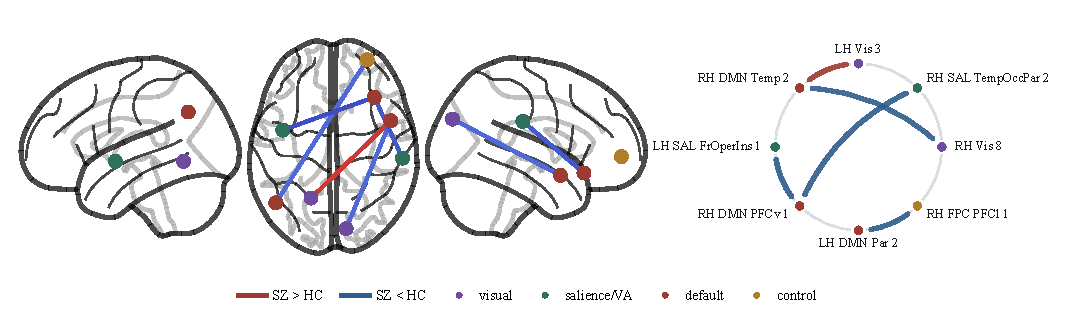
\includegraphics[width=\textwidth]{figures/fig2_connectome.pdf}
\caption{Exploratory connectome of the five edges surviving covariate-adjusted FDR
control, shown on Schaefer-100 centroids (left, sagittal and axial glass-brain
projections) and as a chord diagram (right). The left sagittal view shows no edges
because none of the five surviving connections is confined to the left hemisphere;
three cross the midline (axial view) and two are right--right (right sagittal view).
Warm edges indicate higher connectivity in patients, cool edges lower; line width
scales with the adjusted $t$ statistic. Node colour encodes the Yeo seven-network
assignment.}
\label{fig:connectome}
\end{figure}

\subsection{Leakage-Free Classification}
When no held-out information reaches feature construction, whole-connectome sparse and
component-based representations perform best (Table~\ref{tab:methods},
Fig.~\ref{fig:methods}). PCA-30 with covariates reached $0.771 \pm 0.079$ and the elastic
net $0.768 \pm 0.076$. Their fold distributions overlap almost completely, so we treat
them as equivalent and designate the elastic net as the primary model because it returns
sparse edge weights. Removing the covariate block changes little ($0.765 \pm 0.079$),
which indicates that the imaging features rather than the appended demographics carry the
discrimination. Hard univariate screening ($0.705 \pm 0.071$) and network averaging
($0.679 \pm 0.092$) performed clearly worse. Permutation of the labels placed the null
mean near 0.49 with an empirical $p < 0.02$ at the resolution of 50 shuffles.

\begin{table}[t]
\centering
\caption{Leakage-free benchmark over 50 outer splits (five folds, ten repeats). AUC and
accuracy are fold means $\pm$ standard deviations; the last column pools all out-of-fold
predictions. Standard deviations describe the spread across overlapping repeats and are
not confidence intervals.}
\label{tab:methods}
\begin{tabular}{llrrr}
\toprule
Feature construction & Classifier & AUC & Accuracy & Pooled OOF AUC \\
\midrule
PCA-30 + covariates                  & Logistic    & $0.771 \pm 0.079$ & $0.713 \pm 0.074$ & 0.751 \\
Elastic net, 4,950 edges + covariates & Elastic net & $0.768 \pm 0.076$ & $0.687 \pm 0.076$ & 0.752 \\
Elastic net, edges only              & Elastic net & $0.765 \pm 0.079$ & $0.682 \pm 0.076$ & 0.752 \\
CPM, top/bottom decile + covariates  & Logistic    & $0.742 \pm 0.091$ & $0.680 \pm 0.083$ & 0.733 \\
Top-20 $|t|$ within fold + covariates & Logistic   & $0.705 \pm 0.071$ & $0.641 \pm 0.074$ & 0.693 \\
Network-28 + covariates              & Logistic    & $0.679 \pm 0.092$ & $0.644 \pm 0.079$ & 0.670 \\
\bottomrule
\end{tabular}
\end{table}

\begin{figure}[t]
\centering
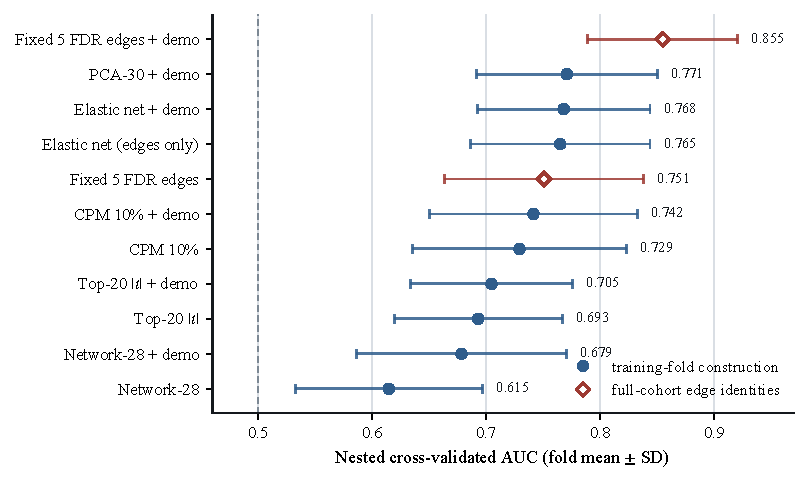
\includegraphics[width=0.84\textwidth]{figures/fig3_methods.pdf}
\caption{Feature-construction strategies under nested cross-validation. Markers give the
fold mean, whiskers one standard deviation across the 50 outer splits. Open diamonds mark
the two settings whose edge identities were fixed on the full cohort and which are
therefore not leakage-free.}
\label{fig:methods}
\end{figure}

\subsection{Isolating the Leakage Effect}
Relaxing fold isolation increases apparent performance (Fig.~\ref{fig:leakage}a).
Freezing the five covariate-adjusted edges lifts the AUC to $0.855 \pm 0.066$ even though
the classifier itself is cross-validated. That setting differs from the primary model in
feature space and classifier as well as in selection scope, so the 0.087 spread is a
mixed-protocol bound rather than leakage in isolation.

The matched contrast removes that ambiguity (Fig.~\ref{fig:leakage}b). With the same
twenty-edge screen, the same logistic classifier and the same grid, computing the screen
inside the training fold yields $0.709 \pm 0.076$, whereas computing it on the complete
cohort yields $0.903 \pm 0.039$. The difference of 0.194 AUC is the cost of leaking this
twenty-edge univariate screen, not the leakage cost of the primary elastic net, which
already shrinks inside the fold and for which we do not report a matched leaked
counterpart. The leakage-free arm here uses three repeats and matches the ten-repeat
value of Table~\ref{tab:methods} (0.705) to within 0.004.

\begin{figure}[t]
\centering
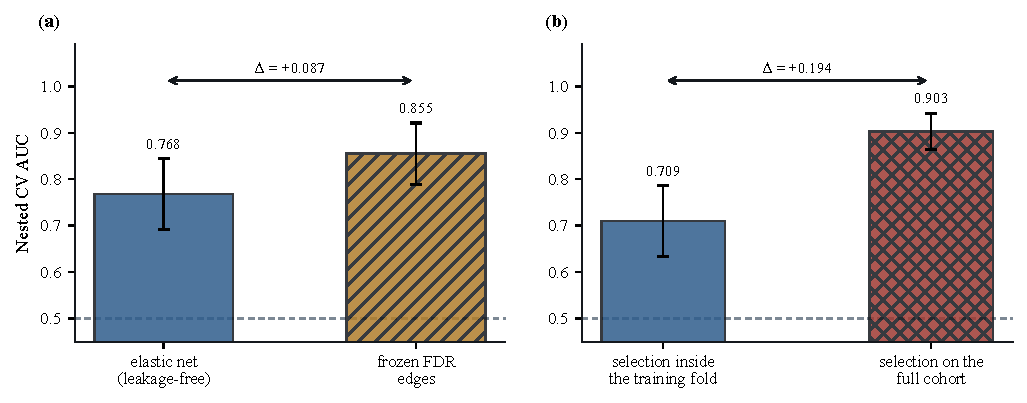
\includegraphics[width=0.92\textwidth]{figures/fig4_leakage.pdf}
\caption{(a) Mixed protocol: freezing the five full-cohort FDR edges raises apparent
performance by 0.087 AUC, but the two settings also differ in feature space and
classifier. (b) Matched contrast: identical top-20 screen, classifier and grid,
differing only in whether the screen sees the test fold. The 0.194 AUC gap is the cost
of leaking this univariate screen, not of leaking the primary elastic net.}
\label{fig:leakage}
\end{figure}

\subsection{Contribution of Head Motion}
Motion is not eliminated by omitting FD from the design matrix. Residualising every edge
on FD within the fold lowers the edges-only elastic net from $0.770 \pm 0.072$ to
$0.694 \pm 0.104$ and the edges-only twenty-edge screen, which excludes the covariate
block and therefore starts from 0.686 rather than the 0.709 of Sect.~3.3, to 0.647
(Fig.~\ref{fig:motion}a). Locked 70/30 splits, in which feature construction never sees
the evaluation set, gave a mean AUC of 0.733 for the elastic net and 0.712 for the
univariate screen (Fig.~\ref{fig:motion}b), consistent with the repeated nested estimate.
Part of the honest signal therefore tracks diagnosis-related movement, and estimates
obtained without motion control should be read accordingly.

\begin{figure}[t]
\centering
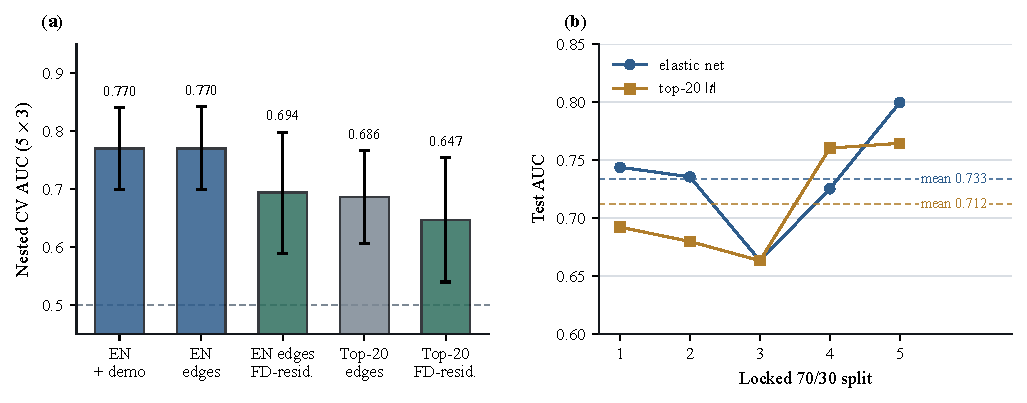
\includegraphics[width=\textwidth]{figures/fig5_motion.pdf}
\caption{(a) Removing mean framewise displacement from every edge within the fold lowers
performance for both the elastic net and univariate screening, indicating that part of
the honest signal is motion-related. (b) Five locked 70/30 splits with all construction
confined to the training portion; dashed lines give the means.}
\label{fig:motion}
\end{figure}

\subsection{Calibration and Aggregation of Repeated Predictions}
For the leakage-free elastic net the expected calibration error was 0.116 with a Brier
score of 0.220 (Fig.~\ref{fig:calibration}a, Table~\ref{tab:calibration}); the model
discriminates above chance but its probabilities would require recalibration before any
decision-support use. The leaked arm of the matched contrast looks better on both counts,
with an expected calibration error of 0.064 and a Brier score of 0.136. That improvement
is itself an artefact: the leaked probabilities are fitted to edges chosen with knowledge
of the very labels against which they are then scored, so calibration diagnostics inherit
the leak and cannot be used to detect it. Good calibration is therefore not evidence that
a pipeline is sound. Averaging the repeated out-of-fold probabilities
within participants before computing a single AUC gave 0.764 for the primary model
against 0.749 when all repeated predictions were pooled as if independent
(Fig.~\ref{fig:calibration}b). The two aggregation rules differ by between 0.014 and
0.026 AUC across the regimes examined, so the choice does not alter the conclusions, but
the subject-level value is the one we report.

\begin{table}[t]
\centering
\caption{Aggregation of repeated out-of-fold predictions and calibration. Pooled AUC
concatenates every fold prediction; subject-level AUC averages the repeated probabilities
of each participant first. ECE is the expected calibration error over ten equal-width
bins. The leaked row is better calibrated than the leakage-free rows, which shows that
calibration cannot diagnose leakage.}
\label{tab:calibration}
\begin{tabular}{lrrrr}
\toprule
Model & Pooled AUC & Subject-level AUC & ECE & Brier \\
\midrule
Elastic net + covariates      & 0.749 & 0.764 & 0.116 & 0.220 \\
Elastic net, edges only       & 0.749 & 0.764 & 0.118 & 0.220 \\
Top-20 $|t|$ inside the fold    & 0.705 & 0.731 & 0.080 & 0.221 \\
Top-20 $|t|$ on the full cohort & 0.884 & 0.904 & 0.064 & 0.136 \\
\bottomrule
\end{tabular}
\end{table}

\begin{figure}[t]
\centering
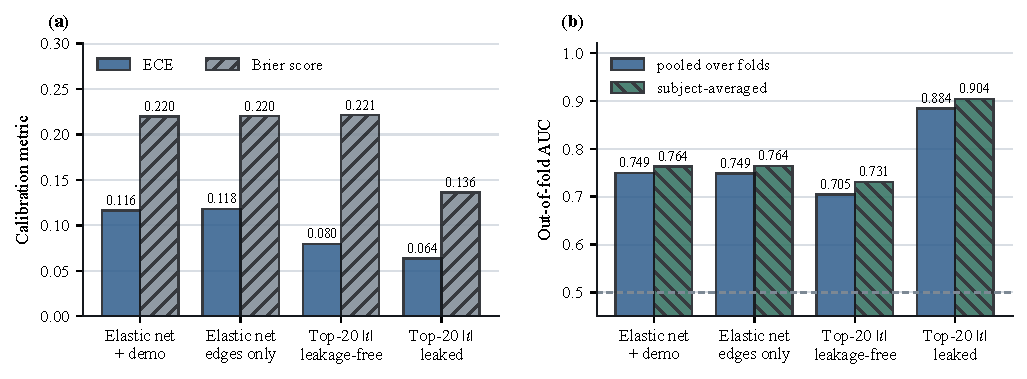
\includegraphics[width=\textwidth]{figures/fig7_calibration.pdf}
\caption{(a) Calibration of the leakage-free models and of the leaked contrast. A leaked
pipeline can be both more discriminative and better calibrated than an honest one, so
neither metric detects the leak. (b) Pooling every repeated out-of-fold prediction
as independent versus averaging the repeated probabilities within each participant before
computing a single AUC.}
\label{fig:calibration}
\end{figure}

\subsection{What the Leaked Reference Model Uses}
Aggregated across outer folds, the largest weight of the leaked reference model is mean
FD ($0.174 \pm 0.125$), followed by the left visual to right default-mode temporal edge
($0.169 \pm 0.103$); all five covariate-adjusted edges recur among the leading
contributors (Fig.~\ref{fig:coefficients}). A motion summary
outranking every connectivity feature in a model whose edges were selected on the full
cohort is a description of the circularity, not a biological result, and we draw no
anatomical inference from it.

\begin{figure}[t]
\centering
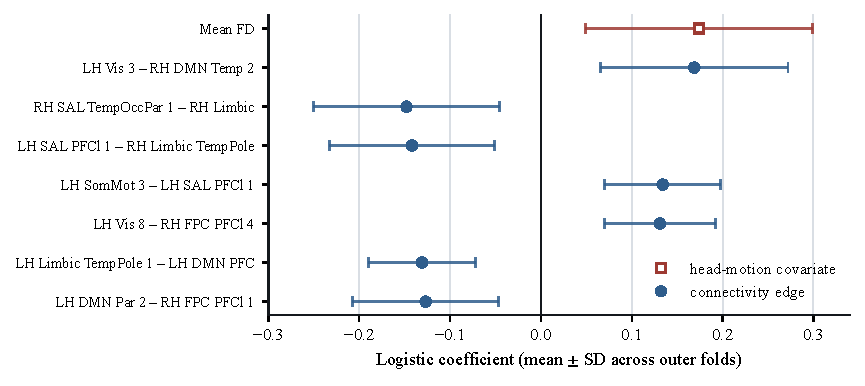
\includegraphics[width=0.78\textwidth]{figures/fig6_coefficients.pdf}
\caption{Largest averaged coefficients of the leaked reference logistic model. Mean
framewise displacement carries the largest weight, which characterises the circular
pipeline rather than the neurobiology of schizophrenia.}
\label{fig:coefficients}
\end{figure}

\subsection{Matched Schizophrenia Sample and Null Control}
On a 50/50 age-, sex- and FD-matched UCLA CNP subsample the same twenty-edge
construction yields $0.679 \pm 0.074$ inside the training fold and
$0.873 \pm 0.081$ on the full subsample (Fig.~\ref{fig:external}b), a gap of 0.194
(five folds, three repeats). A leakage-free logistic model over all 4,950 edges reached
0.727. Accuracy is now interpretable (chance 0.50; leakage-free twenty-edge accuracy
0.617). fMRIPrep and the absence of a locked transfer mean these numbers do not replace
0.77; they show that the 0.194 inflation is not an artefact of COBRE's class balance.

The null control is the more informative extra experiment. On data with no signal the
leakage-free protocol returns chance at the COBRE dimensions
($0.505 \pm 0.068$ independent; $0.516 \pm 0.064$ correlated), which is what an unbiased
estimator must do and which validates the primary design. A leaked twenty-edge screen on
the same data reports $0.821 \pm 0.020$ when edges are correlated as in a connectome and
$0.938 \pm 0.017$ when they are independent. The leaked COBRE value of 0.903 therefore
sits about 0.08 above the correlated floor and 0.03 below the independent ceiling
(Fig.~\ref{fig:external}b): leakage accounts for most of that figure, but the correlated
null does not swallow it entirely. Independent features are an upper bound on
manufacturable optimism, not the reference for a real connectome. On the balanced CNP
connectomes a leaked twenty-edge screen reports 0.873 on synthetic correlated nulls,
0.893 when the observed labels are permuted, and 0.971 on independent features. The
observed leaked value of 0.873 therefore does not exceed the permutation floor: leakage
accounts for that figure, while the leakage-free arm (0.679) remains above chance.
Retaining more edges makes leakage worse: with independent features the leaked AUC rises
from 0.809 at $k = 5$ to 0.937 at 20 and 0.998 at 100 (Fig.~\ref{fig:external}a).
Optimism on null data falls with sample size, from 0.501 at $n = 50$ to 0.263 at 600
(Fig.~\ref{fig:external}c).

\begin{figure}[t]
\centering
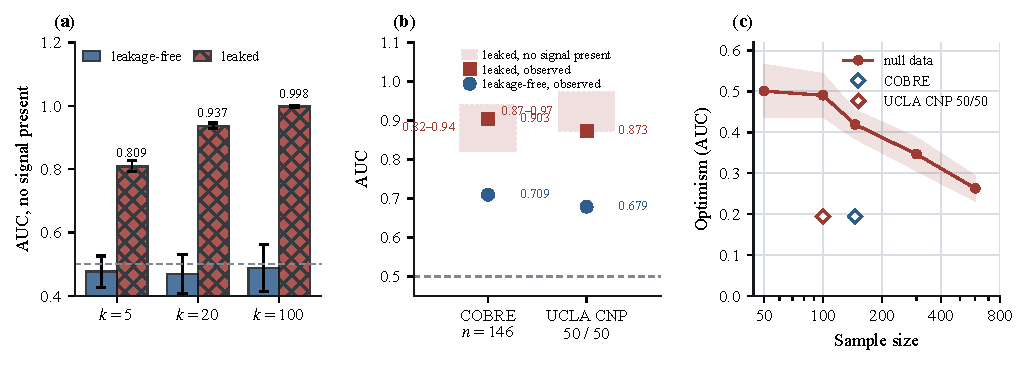
\includegraphics[width=\textwidth]{figures/fig8_external.pdf}
\caption{(a) On data with no signal, a leaked twenty-edge screen reports more the more
edges it retains, while the leakage-free protocol stays at chance. (b) Observed estimates
against the band a leaked twenty-edge screen reaches on signal-free data of the same
dimensions. The lower edge of each band uses correlated connectome edges and is the
relevant floor; the upper edge uses independent features and is an upper bound. COBRE
leaked (0.903) sits about 0.08 above the correlated floor. UCLA CNP is a 50/50 age-,
sex- and FD-matched within-cohort audit under fMRIPrep, not a locked transfer; its leaked
0.873 sits at the correlated floor and does not exceed a label-permutation floor of 0.893.
(c) Optimism against sample size on independent-feature null data.}
\label{fig:external}
\end{figure}

\section{Discussion}

The central observation of this audit is that the same 146 scans support AUCs between
0.71 and 0.90 depending only on when a twenty-edge univariate screen is computed. That
0.194 gap is the price of leaking this construction. It is not the leakage cost of the
primary elastic net, which already shrinks inside the fold. Freezing the five FDR edges
raises the AUC to 0.855, but that comparison also changes the feature space, so it is not
an isolated leakage effect.

The null control sharpens that reading. The relevant reference is a leaked twenty-edge
screen run on signal-free connectomes with realistic edge dependence, which reports 0.821
at the COBRE dimensions. The leaked COBRE value of 0.903 exceeds that floor by about
0.08, so most of the leaked figure is a property of the design, but not all of it.
Independent Gaussian features raise the same screen to 0.938 and should be read as an
upper bound, not as evidence that 0.903 is indistinguishable from noise. A leaked figure
should never be compared against chance; it should be compared against the same pipeline
on label-shuffled or synthetic data of comparable dependence. The leakage-free arm
returning chance on those data is what licenses reading 0.768 as signal.

The UCLA CNP contrast, after 1:1 matching on age, sex and FD, reproduces the same
0.194 gap (0.679 vs 0.873) and does not license reading 0.679 as a replication of 0.77.

The honest estimate itself should be scoped carefully. Roughly 0.77 AUC applies to this
cohort, this parcellation, Pearson connectivity and this family of classical linear and
sparse models; it is not a ceiling for schizophrenia decoding in general, and larger
samples, different connectivity estimators or representation learning may well exceed it.
Published COBRE results between 0.75 and 0.90~\cite{Arbabshirani2017,Wolfers2015} are best
compared only after each study's selection protocol is known.

Feature construction mattered more than the choice of classifier. Regularised models over
the full connectome and low-dimensional projections behaved similarly, while hard
thresholding of univariate statistics lost about six AUC points. With about 117
training participants per split the ranking of individual edges is unstable, so methods
that accumulate many weak effects outperform those that discard them~\cite{Varoquaux2017}.
Since the fold distributions of the leading leakage-free methods overlap, we make no claim
that any one of them is superior.

Motion deserves explicit treatment rather than a footnote. Mean FD differs between groups,
dominates the weights of the circular model, and its fold-wise removal costs about 0.08
AUC. The edges-only model still discriminates, so the result is not reducible to movement,
but a portion of the honest performance is motion-related and this should be stated
whenever connectome classifiers are compared across cohorts with different acquisition
quality.

Several limitations remain. UCLA CNP is a within-cohort fMRIPrep audit on a 50/50
matched subsample, not a locked transfer, and has no fold-wise FD residualisation of
edges. The correlated synthetic null is a five-component latent structure; the tighter
CNP control is a label permutation of the observed matched connectomes. Connectivity is
Pearson correlation, the model family is classical, the permutation test on COBRE
resolves probabilities only to about 0.02, and secondary analyses use three rather than
ten repeats. No motion-matched COBRE subsample was constructed.

\section{Conclusion}

We measured how well resting-state connectomes classify schizophrenia in COBRE when
feature construction is denied access to test labels, and how much that estimate inflates
when access is granted. Under repeated nested cross-validation the honest AUC is
$0.768 \pm 0.076$, while a twenty-edge screen that sees the full cohort reports 0.903,
about 0.08 above the same screen on signal-free connectomes. Four practices follow for
connectome classification: validate the feature-construction step with the same rigour
as the classifier; report leakage as a matched contrast in which only the selection scope
changes; compare any leaked figure with a synthetic or permuted null of comparable
feature dependence, not with chance; and keep exploratory group maps separate from
predictive features. The protocol and all scripts are
available at \url{https://github.com/Ishsirjan/Leakage_Audit}.

\begin{credits}
\subsubsection{\discintname}
The author has no competing interests to declare that are relevant to the content of this
article.
\end{credits}

\bibliographystyle{splncs04}
\bibliography{references}

\end{document}
